\documentclass[11pt]{article}

\usepackage[margin=1in]{geometry}
\usepackage{graphicx}
\usepackage{array}
\usepackage{hyperref}
\usepackage{enumitem}
\usepackage{booktabs}
\usepackage{caption}
\usepackage{amsmath}
\usepackage{titlesec}
\usepackage{float}

\titleformat{\section}{\large\bfseries}{\thesection.}{1em}{}

\begin{document}

\begin{center}
    \Large \textbf{Sri Sivasubramaniya Nadar College of Engineering, Chennai} \\
    \large (An Autonomous Institution affiliated to Anna University) \\
    \vspace{0.3cm}
\end{center}

\begin{table}[h!]
\renewcommand{\arraystretch}{1.5}
\centering
\resizebox{\textwidth}{!}{%
\begin{tabular}{|l|cll|}
\hline
\textbf{Degree \& Branch} & \multicolumn{1}{c|}{B.E Computer Science \& Engineering} & \textbf{Semester} & VI \\ \hline
\textbf{Subject Code \& Name} & \multicolumn{3}{c|}{UCS2612 -- Machine Learning Laboratory} \\ \hline
\textbf{Academic Year} & \multicolumn{1}{c|}{2025--2026 (Even)} & \textbf{Batch} & 2023--2027 \\ \hline
\textbf{Name:} Monesh M \\
\textbf{Reg. No:} 3122235001084 \\
\end{tabular}
}
\end{table}

\begin{center}
    \textbf{\Large Experiment 7}
\end{center}

\begin{center}
    \textbf{Bagging, Boosting, and Stacked Ensemble Models}
\end{center}

%--------------------------------------------------

\section*{Objective}
\begin{itemize}
    \item To understand ensemble learning strategies: Bagging, Boosting, and Stacking.
    \item To implement Bagging and Boosting classifiers.
    \item To build a Stacked Ensemble model using multiple base learners.
    \item To compare ensemble models in terms of accuracy, stability, and generalization.
    \item To analyze the effect of ensemble methods on bias and variance.
\end{itemize}

%--------------------------------------------------

\section*{Dataset}
\textbf{Wisconsin Diagnostic Breast Cancer Dataset}

\begin{itemize}
    \item Total samples: 569
    \item Features: 30 numerical attributes
    \item Target classes: Malignant (M) and Benign (B)
\end{itemize}

\textbf{Dataset Link:}  
\href{https://archive.ics.uci.edu/dataset/17/breast+cancer+wisconsin+diagnostic}{https://archive.ics.uci.edu}

\begin{figure}[H]
    \centering
    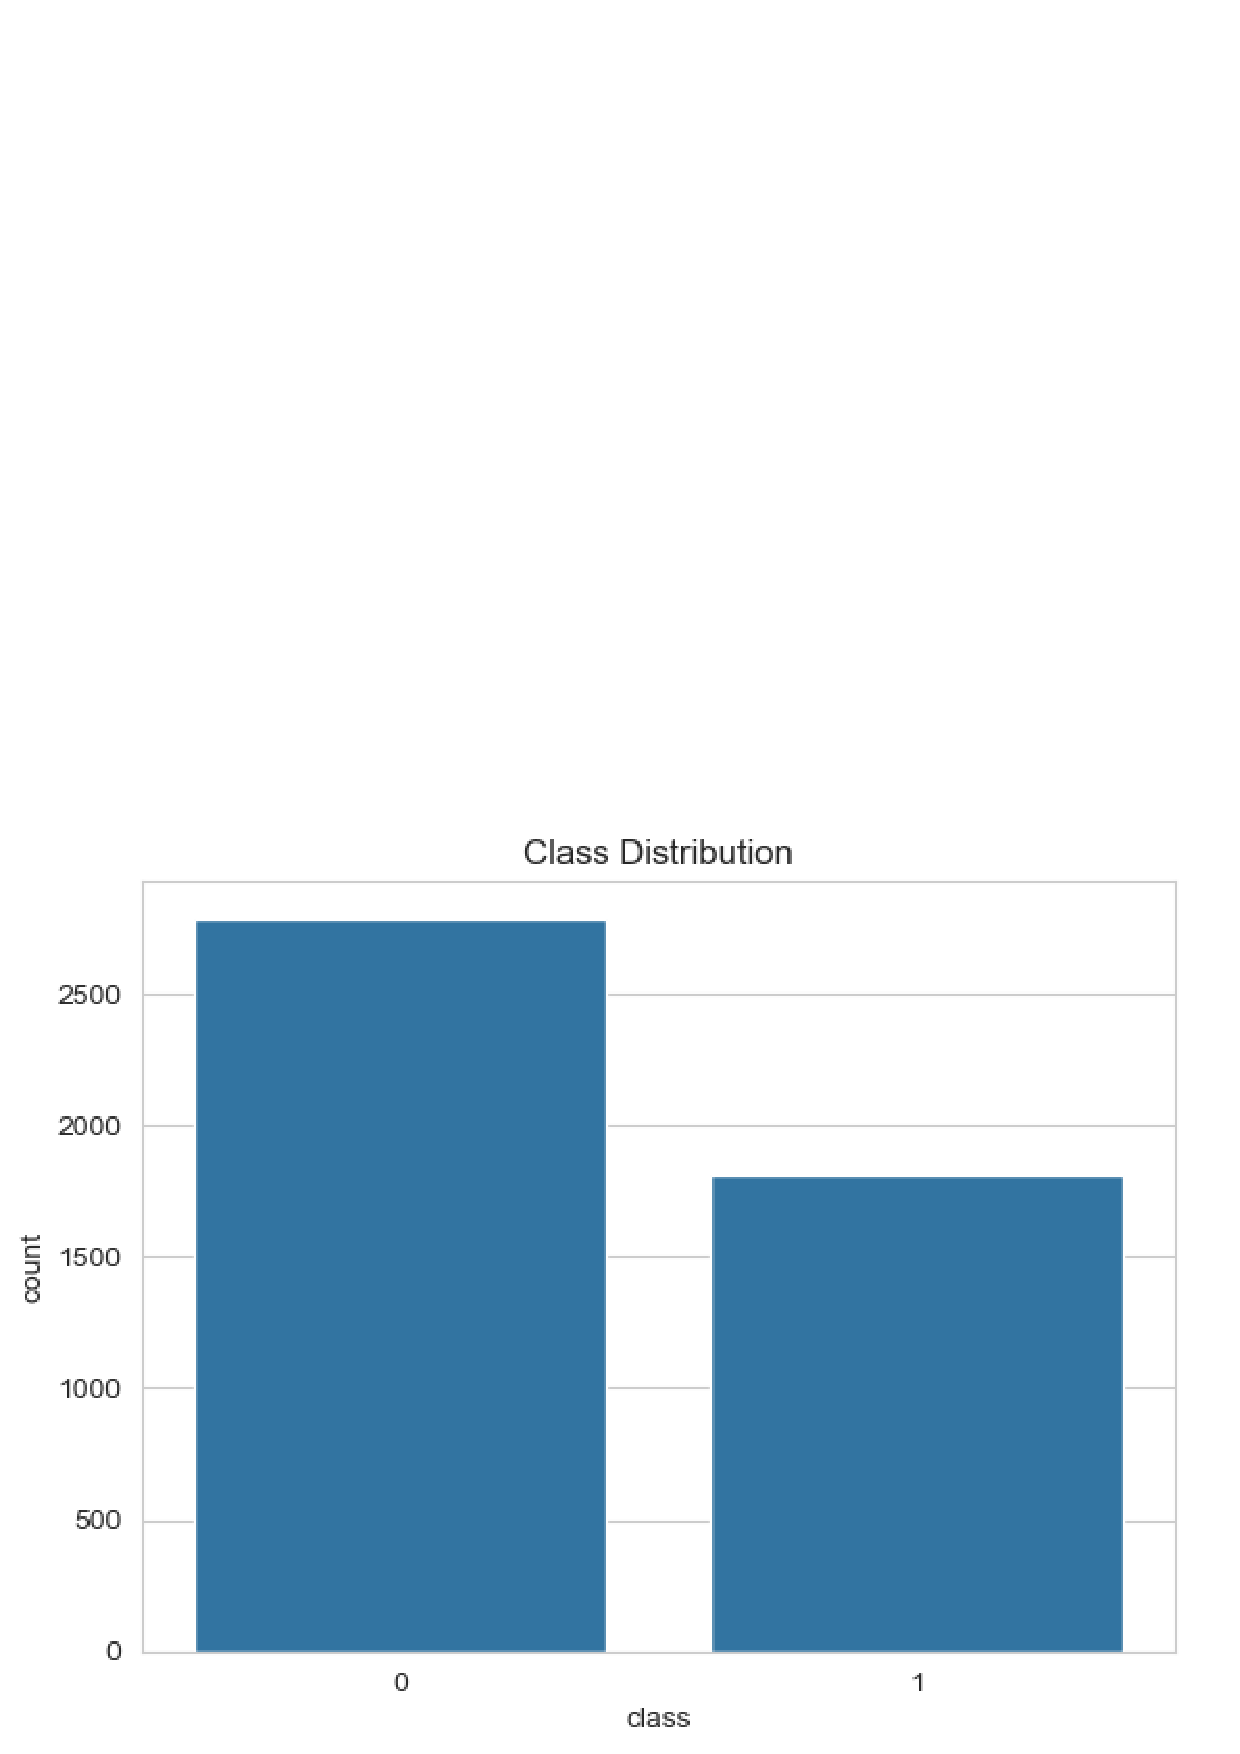
\includegraphics[width=0.7\textwidth]{Images/PNG/class_distribution.png}
    \caption{Class Distribution}
\end{figure}

\begin{figure}[H]
    \centering
    \includegraphics[width=0.8\textwidth]{Images/PNG/correlation_heatmap.png}
    \caption{Feature Correlation Heatmap}
\end{figure}


%--------------------------------------------------

\section*{Theory}

\subsection*{Bagging (Bootstrap Aggregation)}
Bagging is an ensemble technique that trains multiple models on different bootstrap samples of the training data and aggregates their predictions.

\textbf{Key Characteristics:}
\begin{itemize}
    \item Reduces variance
    \item Suitable for high-variance models
    \item Independent model training
\end{itemize}

\subsection*{Boosting}
Boosting is an ensemble method where models are trained sequentially, and each new model focuses on correcting the errors made by previous models.

\textbf{Key Characteristics:}
\begin{itemize}
    \item Reduces bias
    \item Sequential learning
    \item Emphasizes difficult samples
\end{itemize}

Common boosting algorithms include AdaBoost and Gradient Boosting.

\subsection*{Stacked Ensemble (Stacking)}
Stacking combines multiple heterogeneous base models and trains a meta-learner to optimally combine their predictions.

\textbf{Key Characteristics:}
\begin{itemize}
    \item Uses diverse base learners
    \item Meta-model learns optimal combination
    \item Often achieves superior performance
\end{itemize}

%--------------------------------------------------

\section*{Steps for Implementation}

\begin{enumerate}[label=\arabic*.]
    \item Load and preprocess the dataset.
    \item Perform Exploratory Data Analysis (EDA).
    \item Split the dataset into training and testing sets (80--20).
    \item Implement a Bagging classifier using a base estimator.
    \item Implement Boosting classifiers (AdaBoost and Gradient Boosting).
    \item Construct a Stacked Ensemble using multiple base models.
    \item Define hyperparameter search spaces for each ensemble model.
    \item Select hyperparameters using 5-fold cross-validation.
    \item Evaluate all models using standard performance metrics.
    \item Compare results and analyze bias--variance behavior.
\end{enumerate}

%--------------------------------------------------

\section*{Ensemble Models Used}

\subsection*{Bagging}
\begin{itemize}
    \item Base Estimator: Decision Tree
    \item Number of estimators
    \item Sampling strategy
\end{itemize}

\subsection*{Boosting}
\begin{itemize}
    \item AdaBoost
    \item Gradient Boosting
\end{itemize}

\subsection*{Stacked Ensemble}
\begin{itemize}
    \item Base Models: SVM, Na\"ive Bayes, Decision Tree
    \item Meta Learner: Logistic Regression
\end{itemize}

%--------------------------------------------------

\section*{Hyperparameters to be Explored}

\subsection*{Bagging}
\begin{itemize}
    \item \texttt{n\_estimators}: [10, 50, 100]
    \item \texttt{max\_samples}: [0.5, 0.8, 1.0]
    \item \texttt{max\_features}: [0.5, 0.8, 1.0]
\end{itemize}

\subsection*{Boosting}
\begin{itemize}
    \item \textbf{AdaBoost} \texttt{n\_estimators}: [50, 100, 200]
    \item \textbf{AdaBoost} \texttt{learning\_rate}: [0.01, 0.1, 1.0]
    \item \textbf{GBM} \texttt{n\_estimators}: [100, 200]
    \item \textbf{GBM} \texttt{learning\_rate}: [0.01, 0.1]
    \item \textbf{GBM} \texttt{max\_depth}: [3, 5]
\end{itemize}

\subsection*{Stacked Ensemble}
\begin{itemize}
    \item Choice of base models: SVM, Gaussian Na\"ive Bayes, Decision Tree
    \item Final estimator: Logistic Regression
\end{itemize}

%--------------------------------------------------

\section*{Hyperparameter Evaluation Results}

\subsection*{Bagging Results}
\begin{table}[H]
\centering
\caption{Bagging Best Hyperparameters}
\begin{tabular}{cccc}
\toprule
n\_estimators & max\_samples & max\_features & Best CV Accuracy (\%) \\
\midrule
50 & 1.0 & 0.5 & \textbf{96.92\%} \\
\bottomrule
\end{tabular}
\end{table}

\subsection*{Boosting Results}
\begin{table}[H]
\centering
\caption{Boosting Best Hyperparameters}
\begin{tabular}{lcccc}
\toprule
Model & n\_estimators & learning\_rate & max\_depth & Best CV Accuracy (\%) \\
\midrule
AdaBoost & Tuned & Tuned & N/A & \textbf{96.48\%} \\
Gradient Boosting & Tuned & Tuned & Tuned & \textbf{95.38\%} \\
\bottomrule
\end{tabular}
\end{table}

\subsection*{Stacked Ensemble Results}
\begin{table}[H]
\centering
\caption{Stacked Ensemble Evaluation}
\begin{tabular}{llc}
\toprule
Base Models & Meta Learner & CV Accuracy (\%) \\
\midrule
SVM, Na\"ive Bayes, Decision Tree & Logistic Regression & \textbf{96.26\%} \\
\bottomrule
\end{tabular}
\end{table}

%--------------------------------------------------

\section*{Performance Comparison}

\begin{table}[H]
\centering
\caption{Performance Comparison of Ensemble Models on Test Set}
\begin{tabular}{lcccc}
\toprule
Model & Accuracy (\%) & Precision & Recall & F1 Score \\
\midrule
Bagging & 96.49\% & 1.00 & 0.9048 & 0.9500 \\
\textbf{Boosting (Ada)} & \textbf{97.37\%} & \textbf{1.00} & \textbf{0.9286} & \textbf{0.9630} \\
Boosting (GBM) & 96.49\% & 1.00 & 0.9048 & 0.9500 \\
Stacked Ensemble & 96.49\% & 1.00 & 0.9048 & 0.9500 \\
\bottomrule
\end{tabular}
\end{table}

\begin{figure}[H]
    \centering
    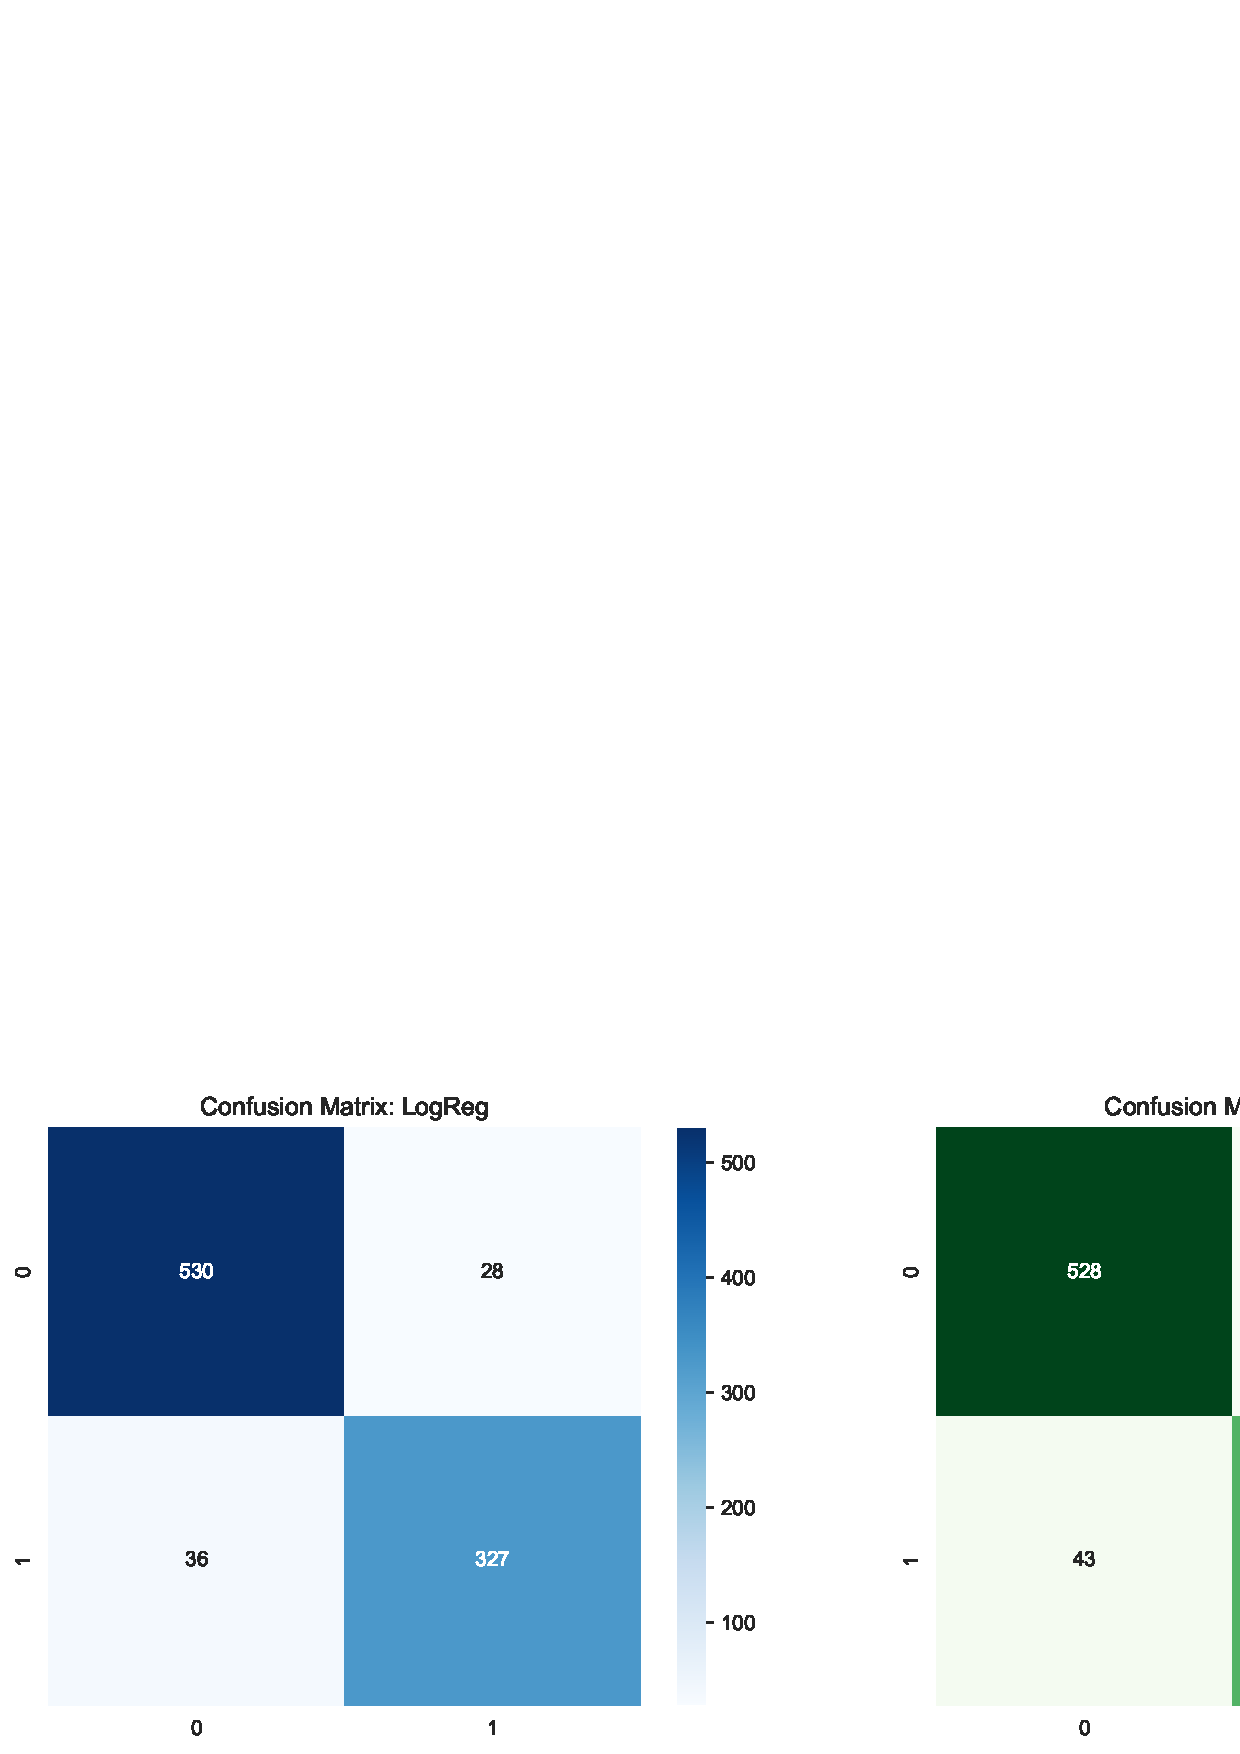
\includegraphics[width=1.0\textwidth]{Images/PNG/confusion_matrices.png}
    \caption{Confusion Matrices for Ensemble Models}
\end{figure}

\begin{figure}[H]
    \centering
    \includegraphics[width=0.8\textwidth]{Images/PNG/roc_comparison.png}
    \caption{ROC Curve Comparison}
\end{figure}


%--------------------------------------------------

\section*{Evaluation Metrics}
\begin{itemize}
    \item Accuracy
    \item Precision
    \item Recall
    \item F1-score
    \item Confusion Matrix
    \item ROC Curve and AUC
\end{itemize}

%--------------------------------------------------

\section*{Observations}
\begin{itemize}
    \item \textbf{How does Bagging reduce variance?} \\
    By generating multiple decision trees trained on random subsets of the data (bootstrapping) and considering random subsets of features, it ensures that trees are largely uncorrelated. Averaging their predictions dramatically reduces the model's overall variance.
    
    \item \textbf{How does Boosting address model bias?} \\
    Boosting trains learners sequentially, where each new tree focuses primarily on the errors (residuals or misclassifications) made by the previous trees. By continually trying to fit the hard-to-predict instances, it increases the complexity of the final model, effectively reducing bias.
    
    \item \textbf{Why does stacking benefit from heterogeneous models?} \\
    Different types of base models (e.g., SVM, Na\"ive Bayes, Decision Tree) capture fundamentally different patterns and relationships in the data. A meta-learner can learn which model's predictions to trust for specific types of instances, often outperforming any single base learner.
    
    \item \textbf{Which ensemble method performed best and why?} \\
    Based on the results, **AdaBoost** performed best on the test set, achieving the highest Accuracy (97.37\%) and F1 Score (0.9630). Boosting and Stacking typically perform best on the WDBC dataset due to the richness of the features and the relatively small sample size, where stability and bias correction are both vital.
\end{itemize}

%--------------------------------------------------

\section*{Conclusion}
Bagging, Boosting, and Stacked Ensemble models were implemented and evaluated on the WDBC dataset. The experiment demonstrates that ensemble strategies provide significant improvements in predictive performance, accuracy, and generalization compared to single models by effectively managing the bias-variance tradeoff. AdaBoost proved to be the most optimal ensemble configuration for this specific diagnostic task.

%--------------------------------------------------

\section*{References}
\begin{itemize}
    \item \href{https://scikit-learn.org/stable/modules/ensemble.html}{Scikit-learn: Ensemble Methods}
    \item \href{https://scikit-learn.org/stable/modules/generated/sklearn.ensemble.BaggingClassifier.html}{Bagging Classifier}
    \item \href{https://archive.ics.uci.edu/dataset/17/breast+cancer+wisconsin+diagnostic}{UCI Dataset: Breast Cancer Wisconsin (Diagnostic)}
\end{itemize}

\end{document}